%% Copernicus Publications Manuscript Preparation Template for LaTeX Submissions
%% ---------------------------------
%% This template should be used for copernicus.cls
%% The class file and some style files are bundled in the Copernicus Latex Package, which can be downloaded from the different journal webpages.
%% For further assistance please contact Copernicus Publications at: production@copernicus.org
%% https://publications.copernicus.org/for_authors/manuscript_preparation.html

%% copernicus_rticles_template (flag for rticles template detection - do not remove!)

%% Please use the following documentclass and journal abbreviations for discussion papers and final revised papers.

%% 2-column papers and discussion papers
\documentclass[gc, manuscript]{copernicus}



%% Journal abbreviations (please use the same for discussion papers and final revised papers)


% Advances in Geosciences (adgeo)
% Advances in Radio Science (ars)
% Advances in Science and Research (asr)
% Advances in Statistical Climatology, Meteorology and Oceanography (ascmo)
% Annales Geophysicae (angeo)
% Archives Animal Breeding (aab)
% ASTRA Proceedings (ap)
% Atmospheric Chemistry and Physics (acp)
% Atmospheric Measurement Techniques (amt)
% Biogeosciences (bg)
% Climate of the Past (cp)
% DEUQUA Special Publications (deuquasp)
% Drinking Water Engineering and Science (dwes)
% Earth Surface Dynamics (esurf)
% Earth System Dynamics (esd)
% Earth System Science Data (essd)
% E&G Quaternary Science Journal (egqsj)
% Fossil Record (fr)
% Geochronology (gchron)
% Geographica Helvetica (gh)
% Geoscience Communication (gc)
% Geoscientific Instrumentation, Methods and Data Systems (gi)
% Geoscientific Model Development (gmd)
% History of Geo- and Space Sciences (hgss)
% Hydrology and Earth System Sciences (hess)
% Journal of Micropalaeontology (jm)
% Journal of Sensors and Sensor Systems (jsss)
% Mechanical Sciences (ms)
% Natural Hazards and Earth System Sciences (nhess)
% Nonlinear Processes in Geophysics (npg)
% Ocean Science (os)
% Primate Biology (pb)
% Proceedings of the International Association of Hydrological Sciences (piahs)
% Scientific Drilling (sd)
% SOIL (soil)
% Solid Earth (se)
% The Cryosphere (tc)
% Web Ecology (we)
% Wind Energy Science (wes)


%% \usepackage commands included in the copernicus.cls:
%\usepackage[german, english]{babel}
%\usepackage{tabularx}
%\usepackage{cancel}
%\usepackage{multirow}
%\usepackage{supertabular}
%\usepackage{algorithmic}
%\usepackage{algorithm}
%\usepackage{amsthm}
%\usepackage{float}
%\usepackage{subfig}
%\usepackage{rotating}

% The "Technical instructions for LaTex" by Copernicus require _not_ to insert any additional packages.
%


\begin{document}

\title{INSYDE: a synthetic, probabilistic flood damage model based on explicit
cost analysis}


\Author[]{}{}



%% The [] brackets identify the author with the corresponding affiliation. 1, 2, 3, etc. should be inserted.



\runningtitle{INSYDE}

\runningauthor{Dottori}





\received{}
\pubdiscuss{} %% only important for two-stage journals
\revised{}
\accepted{}
\published{}

%% These dates will be inserted by Copernicus Publications during the typesetting process.


\firstpage{1}

\maketitle






\section{Introduction}

Flood damage evaluation is a crucial component of any strategy for flood
risk mitigation and management. In particular, models and methodologies
for estimating economic damages are key for evaluating and comparing
flood mitigation measures and for defining flood risk management plans.
Synthetic models adopt a conceptual expert-based approach using
hypotheses and assumptions about damage mechanisms (what-if analysis).
Synthetic damage models can be employed for a variety of applications,
such as the derivation of damage functions for different types of
assets, post-event damage estimation, and analysis of uncertainty
sources in damage assessments. Still, subjectivity in what-if analyses
may result in uncertain damage estimates. In addition, these models are
often affected by a lack of transparency, which limits their
applicability, transferability, and improvements. Indeed, in many cases
the rationale behind model development (e.g.~assumptions, mechanisms
considered, built-in parameters) is not clearly presented and relevant
variables to be used are not well explained. In this paper we propose a
probabilistic methodology to derive synthetic damage curves for
residential buildings called INSYDE (In-depth Synthetic Model for Flood
Damage Estimation). The method is based on an explicit
component-by-component analysis of physical damages to buildings, which
takes into account available knowledge on damage mechanisms. INSYDE is
transparent and applicable to different contexts. Implemented functions
and values are clearly explained so that they can be totally or partly
modified according to the physical context in which the model is
applied. Conversely, the methodology allows for different levels of
detail in the analysis, hence the damage model can be adapted to the
actual knowledge of relevant hazard and vulnerability variables. The
damage functions composing the model have been designed using an
expert-based approach with the support of existing scientific and
technical literature, loss adjustment studies, and damage surveys
carried out for past flood events in Italy. Note: The version in this
paper is limited to residential building damage estimation. It is
important to note that the current version presented in this paper is
limited to residential building damage estimation. The general
methodology, however, can be extended to other types of assets, such as
commercial or industrial buildings.

\section{Model description}

INSYDE adopts a synthetic approach consisting of the simulated,
step-by-step inundation of residential buildings, and in the evaluation
of the corresponding damage based on building and hazard features. Such
a methodology can also be referred to as a what-if analysis. Damages are
first modelled on a component-by-component basis using physically based
mathematical functions and are then converted into monetary terms using
full replacement costs derived from reference price lists. The overall
economic damage to a building is obtained by summing each of the
different damage components: clean-up and removal costs, structural
damage, non-structural damage, damage to finishing elements, damage to
windows and doors, and damage to building systems. For each
subcomponent, a mathematical function describing the damage mechanism
and associated cost is formulated, considering expert-based knowledge as
well as available technical and scientific documentation. The general
formulation can be described as follows: event features include all the
physical variables describing the flood event at the building location,
e.g.~maximum external and internal water depth, flood duration, water
quality (presence of contaminants) and sediment load. Building
characteristics include all the variables that describe features and
geometry of the building. Building features affect damage estimation
either by modifying the functions describing damage mechanisms
(e.g.~system distribution, build- ing structure) or by affecting the
unit prices of the building components by a certain factor
(e.g.~building type, finishing level). Conversely, the geometrical
properties of the building (e.g.~footprint area, number of floors) are
used in the estimation of the extension of damage to each of the
building components. Unit prices refer to the cost of replacement or
reparation of the building components per unit of measure (e.g.~door
removal cost per square metre, pavement replacement cost per square
metre). The cost for each subcomponent is determined by the unit price
(up) and the extension (ext). The latter is the measure of the physical
dimension of the damage (e.g.~m 2 of plaster damaged) and depends on the
event features and building characteristics. This distinction is useful
for model generalization. The extension of the damage is determined only
by the physical effects that the flood event causes to the building;
therefore, the same approach can be applied in different countries or
geographic areas, provided that the local characteristics of the
buildings are accounted for. Unit prices, instead, vary from country to
country or even within a country, they can also be referred to standard
or default unit prices in official publications. Therefore, local price
values are well identified and can be easily replaced with more suitable
ones in this approach. Tables 1 and 2 describe in detail the event
features and building characteristics parameters, their unit of
measurement, their range, and the default values in case no information
is supplied to the model. The variables listed in Tables 1 and 2 can
directly affect damage estimation in terms of extension or indirectly by
influencing other variables. An example of the latter case is YY (year
of construction), which has no direct impact on the damage mechanisms of
the different building subcomponents but indirectly influences the
selection of other variables such as PD (heating system distribution)
and PT (heating system type). Another example is NF (number of floors),
which only directly affects soil consolidation despite indirectly
influencing many other building components because damage on upper
floors can only occur if the floors actually exist in the building. The
number of flooded floors is then calculated as a function of inundation
depth and interfloor height of the building (IH). It is important to
underline that during the model design, observed damage data were
essentially used to analyse the relations between hazard parameters and
damage mechanisms in order to improve physical damage functions. For
instance, the functions for structural damage found in literature were
implemented in the model after some modifications, as they were not in
line with the observed damages. Such a usage is consistent with an
expert-based approach because observed data were first interpreted and
then used to modify parts of the model structure rather than applied to
calibrate the parameters of existing functions. Figure 3 provide an
example of damage functions developed for a default building in the case
of a flood with a duration d = 24 h, flow velocity v = 2.0 m/s, sediment
concentration s = 0.05, and presence of pollutants (q = 1).

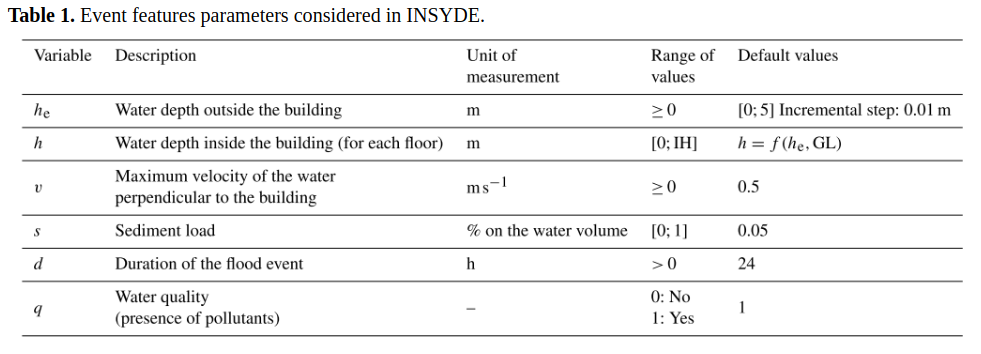
\includegraphics[width=16cm]{table1}

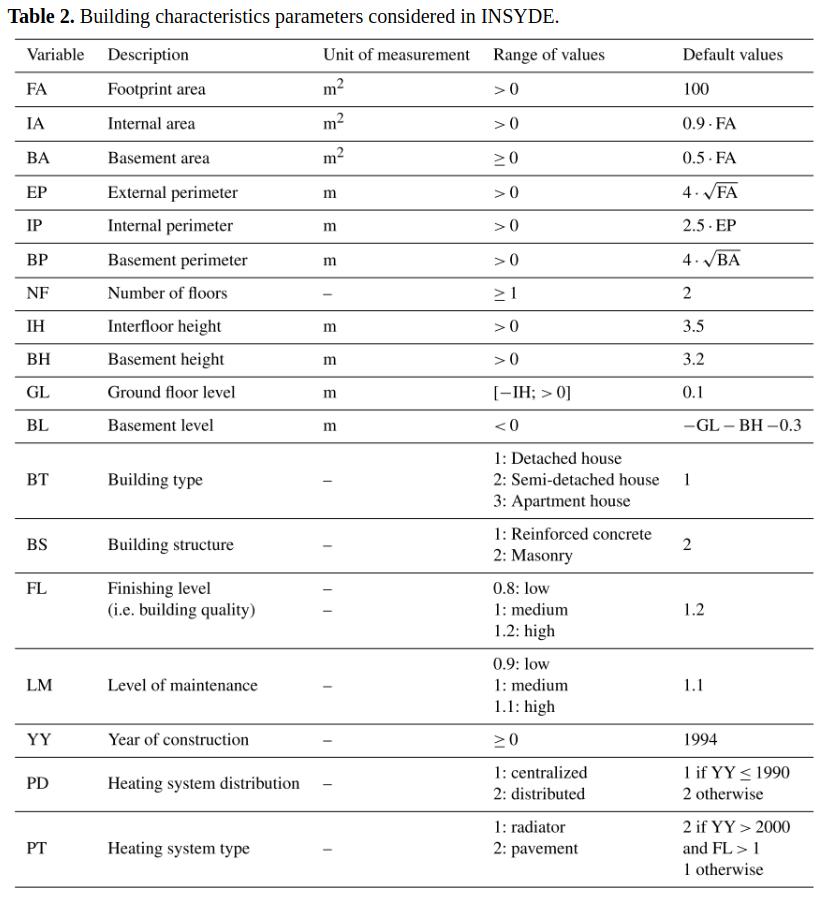
\includegraphics[width=13cm]{table2}

\begin{figure}
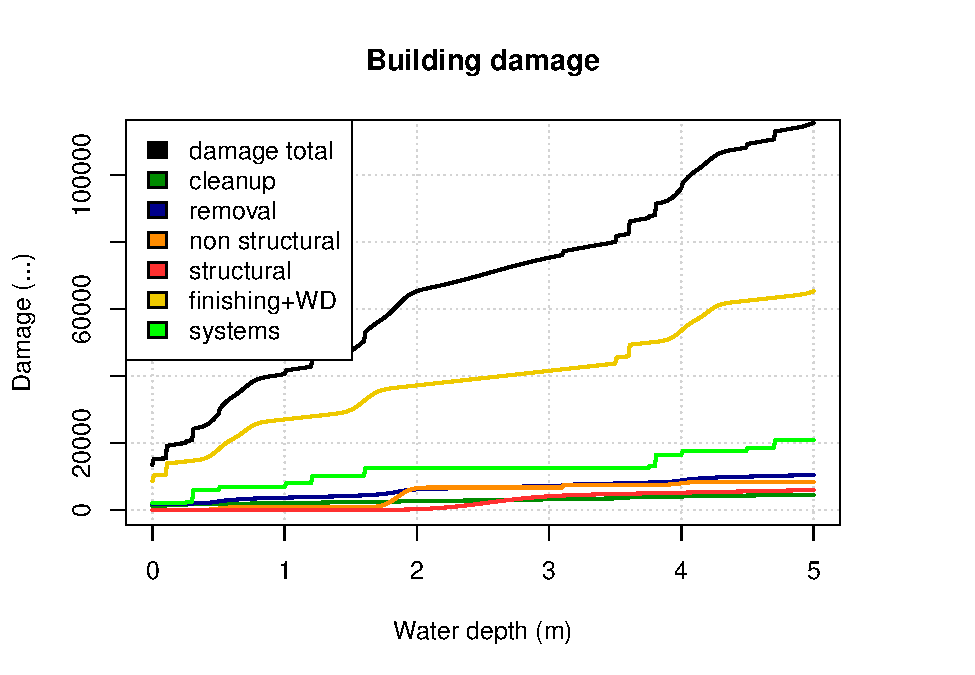
\includegraphics[width=300px]{Insyde_files/figure-latex/clam_setup-1} \caption{Example of INSYDE damage functions considering the following event variables: flow velocity = 2.0 m/s , flood duration = 24 h, sediment concentration = 0.05, and water quality = presence of pollutants (1=yes, 0=no). Damage functions for entire building and different building components.}\label{fig:clam_setup}
\end{figure}

\section{Sensitivity analysis}

To further explore the importance of each of these parameters
(i.e.~water depth, flow velocity, and sediment load), we performed a
local sensitivity analysis. In this application, the damage was computed
by varying alternately each hazard parameter while the others were kept
constant. The building characteristics variables have not been analysed
at this stage. Two different flood conditions have been considered to
explore the model behaviour in different conditions: a low velocity,
long duration flood and, conversely, a high velocity, short duration
flood event. For the first case, the fixed values of depth, velocity,
duration, and sediment load were respectively h = 1.5 m, v = 1.0 m/s, d
= 24 h and s = 0.10. For the second case, the values were h = 2.0 m, v =
2.0 m/s, d = 10 h and s = 0.10. Computations were performed considering
a standard reinforced concrete building with two floors and a basement,
100m\^{}2 of floor area, and a high finishing level. The other building
characteristics were set using the previously mentioned default values.
Figures 2 and 3 summarize the results of the local sensitivity analysis
in the two chosen flood conditions, showing the relative influence of
each hazard variable in determining the total economic damage. As
expected, water depth is the most influential parameter since all the
damage functions directly depend on it. Relative changes in flood
duration have much more impact in low velocity, long duration events,
while the relevance of velocity is more evident at higher values, when
structural damages can become important. In both scenarios sediment load
has a relatively marginal importance. The influence of water quality q
is not included in Figs. 2 and 3 because it is a binary variable and,
therefore, cannot be increased or decreased incrementally and directly
compared with the other variables. Both base cases were thus computed
considering the absence of pollutants (q = 0). To illustrate the
influence of this hazard variable on model results, we computed the same
two base cases separately considering the presence of pollutants (q =
1). The resulting relative increase in damage for the presence of
pollutants ranges from around 30 to 45 \%.

\begin{figure}
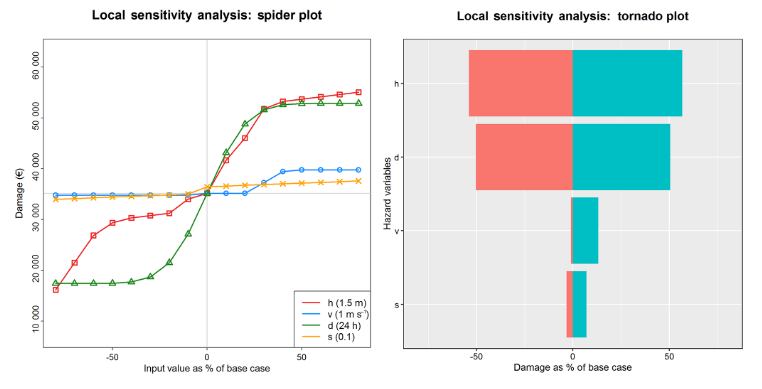
\includegraphics[width=13cm]{fig2} \caption{Results of the local sensitivity analysis in case of low velocity, long duration flood.}\label{fig:unnamed-chunk-3}
\end{figure}

\begin{figure}
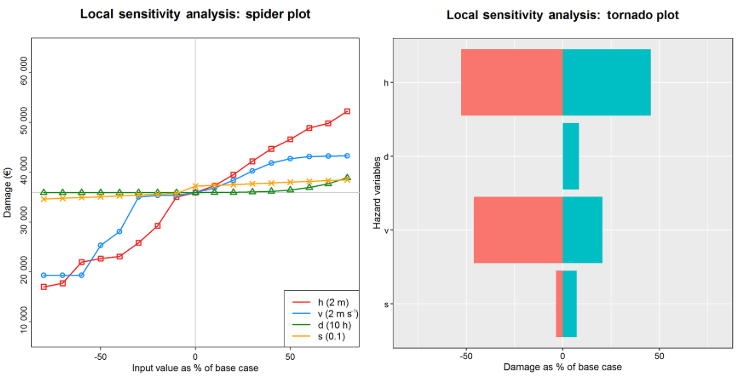
\includegraphics[width=13cm]{fig3} \caption{Results of the local sensitivity analysis in the case of high velocity, short duration flood.}\label{fig:unnamed-chunk-4}
\end{figure}







%%%%%%%%%%%%%%%%%%%%%%%%%%%%%%%%%%%%%%%%%%
%% optional

%%%%%%%%%%%%%%%%%%%%%%%%%%%%%%%%%%%%%%%%%%

%%%%%%%%%%%%%%%%%%%%%%%%%%%%%%%%%%%%%%%%%%

%%%%%%%%%%%%%%%%%%%%%%%%%%%%%%%%%%%%%%%%%%
\competinginterests{} %% this section is mandatory even if you declare that no competing interests are present

%%%%%%%%%%%%%%%%%%%%%%%%%%%%%%%%%%%%%%%%%%

%%%%%%%%%%%%%%%%%%%%%%%%%%%%%%%%%%%%%%%%%%

%% REFERENCES
%% DN: pre-configured to BibTeX for rticles

%% The reference list is compiled as follows:
%%
%% \begin{thebibliography}{}
%%
%% \bibitem[AUTHOR(YEAR)]{LABEL1}
%% REFERENCE 1
%%
%% \bibitem[AUTHOR(YEAR)]{LABEL2}
%% REFERENCE 2
%%
%% \end{thebibliography}

%% Since the Copernicus LaTeX package includes the BibTeX style file copernicus.bst,
%% authors experienced with BibTeX only have to include the following two lines:
%%
\bibliographystyle{copernicus}
\bibliography{}
%%
%% URLs and DOIs can be entered in your BibTeX file as:
%%
%% URL = {http://www.xyz.org/~jones/idx_g.htm}
%% DOI = {10.5194/xyz}


%% LITERATURE CITATIONS
%%
%% command                        & example result
%% \citet{jones90}|               & Jones et al. (1990)
%% \citep{jones90}|               & (Jones et al., 1990)
%% \citep{jones90,jones93}|       & (Jones et al., 1990, 1993)
%% \citep[p.~32]{jones90}|        & (Jones et al., 1990, p.~32)
%% \citep[e.g.,][]{jones90}|      & (e.g., Jones et al., 1990)
%% \citep[e.g.,][p.~32]{jones90}| & (e.g., Jones et al., 1990, p.~32)
%% \citeauthor{jones90}|          & Jones et al.
%% \citeyear{jones90}|            & 1990

\end{document}
